\documentclass{beamer}
\usetheme[pageofpages=de,% String used between the current page and the
                         % total page count.
          bullet=circle,% Use circles instead of squares for bullets.
          titleline=true,% Show a line below the frame title.
          alternativetitlepage=true,% Use the fancy title page.
          titlepagelogo=../img/fse_ministerio_ancho_texto.png%,% Logo for the first page.
	  %watermark=junta_girado,
          %watermarkheight=75px,% Height of the watermark.
          %watermarkheightmult=4,% The watermark image is 4 times bigger
                                % than watermarkheight.
          ]{Torino}

\usepackage[spanish]{babel} % Para separar correctamente las palabras
\usepackage[utf8]{inputenc} % Este paquete permite poner acentos y eñes usando codificación utf-8

\usepackage{color}

\author{
\small{IES Gonzalo Nazareno}\\
\tiny{Dos Hermanas (Sevilla)}\\
\small{IES Los Albares}\\
\tiny{Cieza (Murcia)}\\
\small{IES La Campiña}\\
\tiny{Arahal (Sevilla)}\\
\small{IES Ingeniero de la Cierva}\\
\tiny{Murcia}\\
\vspace{.5cm}

\includegraphics[width=0.2\textwidth]{cc_by_sa.png}}
\title{IaaS en los estudios de informática}
\institute{Proyecto de Innovación\\ {\color{white} .\\} \emph{Implantación y
    puesta a punto de la infraestructura de un cloud computing privado para el
    despliegue de servicios en la nube}}  

\begin{document}
\setlength{\parskip}{.2cm}

\begin{frame}[t,plain]
\titlepage
\end{frame}

\begin{frame}
  \frametitle{Cloud Computing}
  Tradicionalmente se definen tres capas:
  \begin{description}
  \item[Software as a Service (SaaS)] Aplicación completa ofrecida
    como servicio en la nube (Servicios de Google, Salesforce.com, Microsoft
    Office 365, \ldots)
  \item[Platform as a Service (PaaS)] Aplicación completa para el
    desarrollo ofrecida como servicio en la nube (Google App Engine,
    Windows Azure, RedHat OpenShift, \ldots)
  \item[Infrastructure as a Service (IaaS)] Almacenamiento (también
    denominado \textit{Storage as a Service}) y capacidades de cómputo
    (máquinas completas) ofrecida como servicio en la nube.
  \end{description}
Aquí nos centraremos en la utilización de IaaS en las enseñanzas de informática
\end{frame}

\begin{frame}
  \frametitle{Tipos de IaaS}
  \begin{description}
  \item[Público] Una empresa ofrece IaaS a terceros, encargándose de
    toda la gestión del Cloud. El caso más conocido es Amazon Elastic
    Cloud Computing (EC2).
  \item[Privado] Una organización configura sus propios recursos como
    IaaS para tener más flexibilidad y control total sobre sus
    recursos.
  \item[Híbrido] Algunos servicios se gestionan en el cloud privado y
    otros se transfieren a uno público, normalmente utilizan una API
    común que permita una buena integración.
  \end{description}
\end{frame}

\begin{frame}
  \frametitle{Software para IaaS}
  Hay bastantes opciones, quizás las más relevantes sean:
  \begin{description}
  \item[Privativo]
  \end{description}
  \begin{center}
    
\includegraphics[height=1cm]{../img/vcloud.png}
  \end{center}
  \begin{description}
  \item[Libre]
  \end{description}
  \begin{columns}
    \column{.5\textwidth}
    \begin{center}
      
\includegraphics[height=1.5cm]{../img/eucalyptus.png}\\
      \vspace{.5cm}
      
\includegraphics[height=.75cm]{../img/opennebula.png}
    \end{center}
    \column{.5\textwidth}
    \begin{center}
      
\includegraphics[height=1.5cm]{../img/openstack.jpg}\\
      \vspace{.5cm}
      
\includegraphics[height=1cm]{../img/cloudstack.png}      
    \end{center}
  \end{columns}
\end{frame}

\begin{frame}
  \frametitle{Cloud de infraestructura privado con software libre}
  La mejor opción para utilizar en un entorno educativo es un cloud de
  infraestructura privado basado en software libre
  \begin{description}
  \item[¿Por qué privado?] Permite control total sobre el cloud,
    utilizarlo sin límites y conocerlo de forma detallada.
  \item[¿Por qué libre?] Entre otros motivos:
    \begin{itemize}
    \item Permite control total sobre software
    \item Garantiza la independencia tecnológica
    \item Utiliza estándares
    \item Interoperabilidad
    \item Ahorro de costes
    \end{itemize}
  \end{description}
Las dos opciones más interesantes actualmente son OpenStack y OpenNebula
\end{frame}

\begin{frame}
  \frametitle{Evolución metodológica}
  Antes de ver las posibilidades que ofrece la utilización de IaaS en las
  enseñanzas de informática, vamos a recapitular las fases por las que han
  pasado estas enseñanzas\footnote{Nos referimos siempre a enseñanzas prácticas,
  no a la tiza ;)}
  \begin{itemize}
  \item A la par de la evolución tecnológica, se ha producido una evolución en
    los métodos de enseñanza de informática, que podríamos de forma muy general
    separar en 3 fases:
    \begin{itemize}
    \item Primera fase: Utilización de equipos físicos
    \item Segunda fase: Utilización de máquinas virtuales
    \item Tercera fase: Utilización de IaaS
    \end{itemize}
  \item Estas fases no son excluyentes: una fase siempre puede incluir las
    anteriores.
  \item Todas tienen ventajas e inconvenientes, pero la tercera fase ofrece
    escenarios imposibles de utilizar anteriormente.

  \end{itemize}
\end{frame}

\begin{frame}
  \frametitle{Evolución metodológica. Primera fase}
  \begin{columns}
    \column{.6\textwidth}
    \begin{itemize}
    \item Utilización de máquinas físicas
      \begin{itemize}
      \item Una máquina por alumno
      \item Algunos servidores compartidos
      \end{itemize}
      \item Pros:
      \begin{itemize}
      \item Fácil despliegue y puesta en marcha
      \end{itemize}
      \item Contras:
      \begin{itemize}
      \item Prácticas muy limitadas por número de equipos y tipo de
        configuraciones
      \item Hardware poco variado
      \item Prácticas muy ``académicas''
      \item Muchos tiempos muertos entre prácticas
      \end{itemize}
    \end{itemize}
    \column{.4\textwidth}
    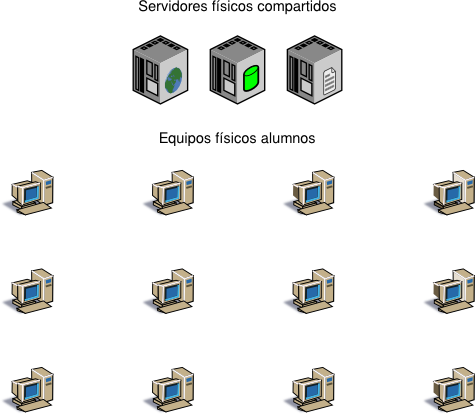
\includegraphics[width=\columnwidth]{../img/epoca1.png}
  \end{columns}
\end{frame}

\begin{frame}
  \frametitle{Evolución metodológica. Segunda fase}
  \begin{columns}
    \column{.6\textwidth}
    \begin{itemize}
    \item Utilización de máquinas virtuales
      \begin{itemize}
      \item Una máquina por alumno
      \item Varias máquinas virtuales por máquina física
      \end{itemize}
      \item Pros:
      \begin{itemize}
      \item Cada alumno dispone de un entorno ``completo'' e independiente
      \item Prácticas menos rígidas
      \item Se aprende virtualización de forma transversal
      \end{itemize}
      \item Contras:
      \begin{itemize}
      \item Entorno más complejo
      \item Requiere equipos actualizados para los alumnos
      \item Los alumnos tienen que administrar el gestor de máquinas
        virtuales 
      \end{itemize}
    \end{itemize}
    \column{.4\textwidth}
    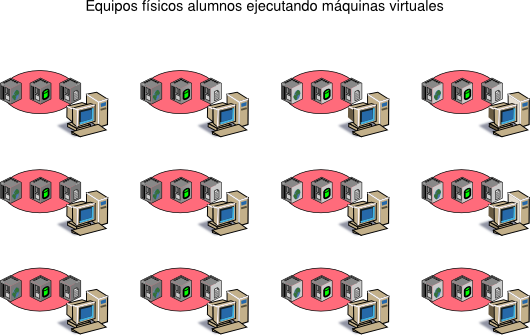
\includegraphics[width=\columnwidth]{../img/epoca2.png}
  \end{columns}
\end{frame}

\begin{frame}
  \frametitle{Evolución metodológica. Tercera fase}
  \begin{columns}
    \column{.6\textwidth}
    \begin{itemize}
    \item Utilización de IaaS
      \begin{itemize}
      \item Un equipo convencional por alumno
      \item IaaS privado de la organización
      \end{itemize}
      \item Pros:
      \begin{itemize}
      \item Enorme variedad de prácticas
      \item Utilización de entornos preconfigurados
      \item Simulación de entornos reales complejos
      \item Equipos básicos para los alumnos
      \item Se aprende IaaS de forma transversal
      \end{itemize}
      \item Contras:
      \begin{itemize}
      \item Sistema muy centralizado
      \item Imprescindible administración del Cloud
      \item Inversión inicial importante
      \end{itemize}
    \end{itemize}
    \column{.4\textwidth}
    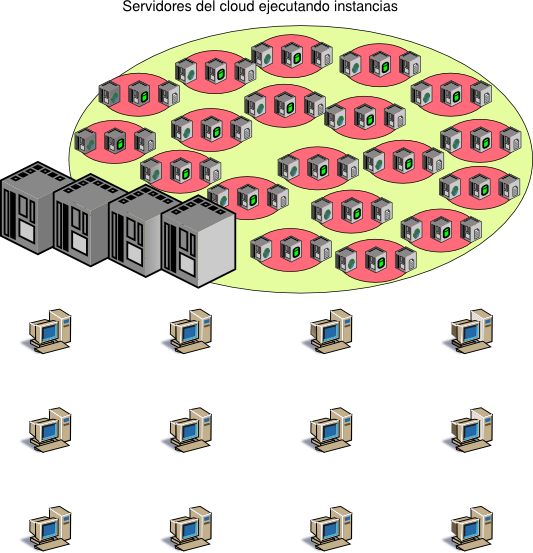
\includegraphics[width=\columnwidth]{../img/epoca3.png}
  \end{columns}
\end{frame}

\begin{frame}
  \frametitle{Simulación de entornos reales}
  Un entorno real es difícil de simular con MVs en un PC por sus
    propias limitaciones, pero en un cloud es asumible:
    \begin{itemize}
    \item Se puede simular una red con un número importante de equipos
    \item Se puede utilizar la diversidad que se quiera de SOs
    \item Este entorno ``real'' pueden utilizarlo conjuntamente todos los
      alumnos
    \item Puede estar disponible durante todo el curso sin interferir con otras
      asignaturas
    \item Con el tiempo y el uso irán apareciendo conflictos y problemas reales
    \end{itemize}
\end{frame}
\begin{frame}
  \frametitle{Nueva forma de aprendizaje}
  \begin{itemize}
  \item La utilización de IaaS en el ámbito académico conlleva una nueva forma
    de aprender
  \item Con el uso de MVs se había impuesto una forma de aprender que no era
    siempre la mejor, por ejemplo:
    \begin{itemize}
    \item Para utilizar un SGBD había que instalarlo y configurarlo antes
    \item Para desplegar una aplicación web, había que configurar previamente
      todo el servidor de aplicaciones
    \item Para hacer prácticas de ZFS había que instalar Solaris o FreeBSD
    \end{itemize}
    \item Un cloud puede contar con gran cantidad de imágenes preconfiguradas de
      sistemas con muy diversas configuraciones $\Rightarrow$ La forma de
      aprender no viene condicionada por la necesidad de una configuración
      previa, por ejemplo:
      \begin{itemize}
      \item Primero se utiliza el SGBD durante varias clases.
      \item Posteriormente, cuando sea oportuno, se aprende a instalarlo y
        configurarlo
      \end{itemize}
  \end{itemize}
\end{frame}

\begin{frame}
  \frametitle{Escenarios (I)}
  \begin{description}
  \item[Instalación y configuración de un servicio]
  \end{description}
  Los pasos típicos a seguir serían:
  \begin{itemize}
  \item Cada alumno inicia una instancia del SO en el que va a instalar el
    servicio (no es necesario que previamente sepa instalar ese SO).
  \item Realiza la instalación del servicio
  \item Realiza la configuración del servicio. Si esta configuración dura
    más de una clase, suspende la instancia y la reinicia en la siguiente
    clase.
  \item Una vez terminada la configuración puede crear una instantánea para
    utilizarla como base en posteriores prácticas.
  \item Si algún alumno no ha podido realizar la configuración correctamente
    podrá utilizar la instantánea de un compañero en clases posteriores.
  \end{itemize}
\end{frame}

\begin{frame}
  \frametitle{Escenarios (II)}
  \begin{description}
  \item[Despliegue de una aplicación web]
  \end{description}
  Los pasos típicos a seguir serían:
  \begin{itemize}
  \item Se prepara una imagen de un sistema en el que se configura de forma
    precisa un completo servidor web con todos los módulos necesarios. Se
    instala y configura un servidor git u otro scm.
  \item Cada alumno inicia una instancia de la imagen anterior y transfiere la
    aplicación web desde su equipo.
  \item Comprueba el funcionamiento en un servidor remoto (la instancia) con
    similares características que tendría en un servidor remoto real.
  \item En caso de que tenga que utilizar la instancia durante más de una clase,
    suspende y reinicia cuando sea necesario.
  \item En caso de fallos o errores, puede crear una nueva instancia a partir de
    la imagen inicial o de una instantánea guardada previamente.
  \end{itemize}
\end{frame}

\begin{frame}
  \frametitle{Escenario (III)}
  \begin{description}
  \item[Utilización de herramientas de sistemas]
  \end{description}
  \begin{itemize}
  \item Se prepara una imagen del sistema que se quiera utilizar, por ejemplo
    una imagen de un SO con soporte ZFS.
  \item Cada alumno inicia una instancia de la imagen anterior sin necesidad de
    saber previamente cómo se instala.
  \item Se asocian a la instancia varios volúmenes volátiles.
  \item Se realizan prácticas de ZFS con los volúmenes anteriores.
  \item Cuando se dominen las herramientas se plantea una instalación del SO
    sobre ZFS
  \end{itemize}
\end{frame}

\begin{frame}
  \frametitle{Escenarios. Resumen}
  \begin{itemize}
  \item Esto no son más que tres ejemplos suficientemente diferentes para ver
    las enormes posibilidades que se abren.
  \item En general, pueden plantearse prácticas más complejas, inviables en el
    esquema tradicional de uso de máquinas virtuales por la complejidad de
    configurar el escenario inicial y por los problemas que acarrea una
    equivocación del alumno durante el desarrollo de la práctica.
  \item Además las prácticas no interfieren con otras asignaturas, parar la
    práctica y continuar otro día es tan simple como suspender la instancia y
    reanudarla cuando se precise.
  \end{itemize}
\end{frame}

\begin{frame}
  \frametitle{Aprendizaje transversal}
  \begin{itemize}
  \item El hecho de utilizar IaaS no como fin en sí mismo sino como herramienta
    para aprender otros temas provoca que el alumno se familiarice fácilmente
    con la tecnología.
  \item Este aprendizaje adquirido de forma continua es mucho más significativo
    que si se impartiera como un tema en una asignatura.
  \item En la mayoría de los casos es suficiente con esto, salvo en los
    estudiantes de Administración de Sistemas, que necesariamente tendrán que
    profundizar más en la materia.
  \end{itemize}
\end{frame}

\begin{frame}
  \frametitle{Administración del Cloud}
  \begin{itemize}
  \item La administración de los sistemas y en particular del cloud de
    una organización no siempre se valora adecuadamente.
  \item La instalación, configuración y administración del cloud es
    una tarea compleja $\Rightarrow$ exige personal cualificado y con
    suficiente dedicación. 
  \item El cloud privado se convierte en el elemento fundamental para
    el desarrollo de prácticas, esto puede suponer un inconveniente en
    caso de errores y hay que planificar alternativas para momentos
    puntuales.
  \end{itemize}
\end{frame}

\begin{frame}
  \frametitle{Inversión inicial}
  \begin{itemize}
  \item Al opta por software libre, la principal inversión son los servidores
    que formarán el cloud de infraestructura.
  \item \textbf{Configuración mínima}: 3 servidores (1 gestión del cloud y 2 para
    ejecución de instancias)
  \item \textbf{Configuración recomendada}: 2 servidores para gestión (en HA), 1
    para almacenamiento y 4 o más para ejecución de instancias
  \item Para la gestión del cloud es suficiente un equipo de características
    mínimas.
  \item Para la ejecución de instancias es necesario procesadores potentes y
    mucha memoria RAM (entre 0,5 y 2 GiB por instancia)
  \item El almacenamiento depende del número de imágenes, instantáneas y
    volúmenes que sea necesario guardar.
  \item Sistema fácilmente escalable, se puede empezar por una
    configuración mínima e ir añadiendo componentes año a año.
  \end{itemize}
\end{frame}

\begin{frame}
  \frametitle{Conclusiones}
  \begin{itemize}
  \item Es necesario incluir Cloud computing en los currículos
  \item No sólo es importante conocer el Cloud, sino que utilizarlo
    habitualmente en clase permite adquirir unas destrezas significativas en su
    manejo
  \item Todas las capas de Cloud son interesantes, pero la que ofrece mayores
    opciones es IaaS
  \item Una organización que implante un cloud de infraestructura propiciará que
    sus alumnos hagan prácticas muy interesantes, difícilmente realizables en
    otros entornos
  \item En el caso de alumnos de sistemas, disponer de un cloud de
    infraestructura, permite conocer con detalle y en profundidad una tecnología
    para la que se prevé una importante demanda futura
  \end{itemize}
\end{frame}
\end{document}
